\documentclass[12pt, landscape]{amsart}
\usepackage[letterpaper, bottom=3cm]{geometry}

\textwidth      =  8.5in
\textheight     =  8.25in
\oddsidemargin  =  18pt
\evensidemargin =  18pt
\topmargin      =  -0.9in


\usepackage[utf8]{inputenc}
\usepackage[spanish]{babel}
\usepackage{anyfontsize}
\usepackage{xcolor}

\usepackage[pages=some]{background}
\backgroundsetup{
scale=1,
color=black,
opacity=1,
angle=0,
contents={%
  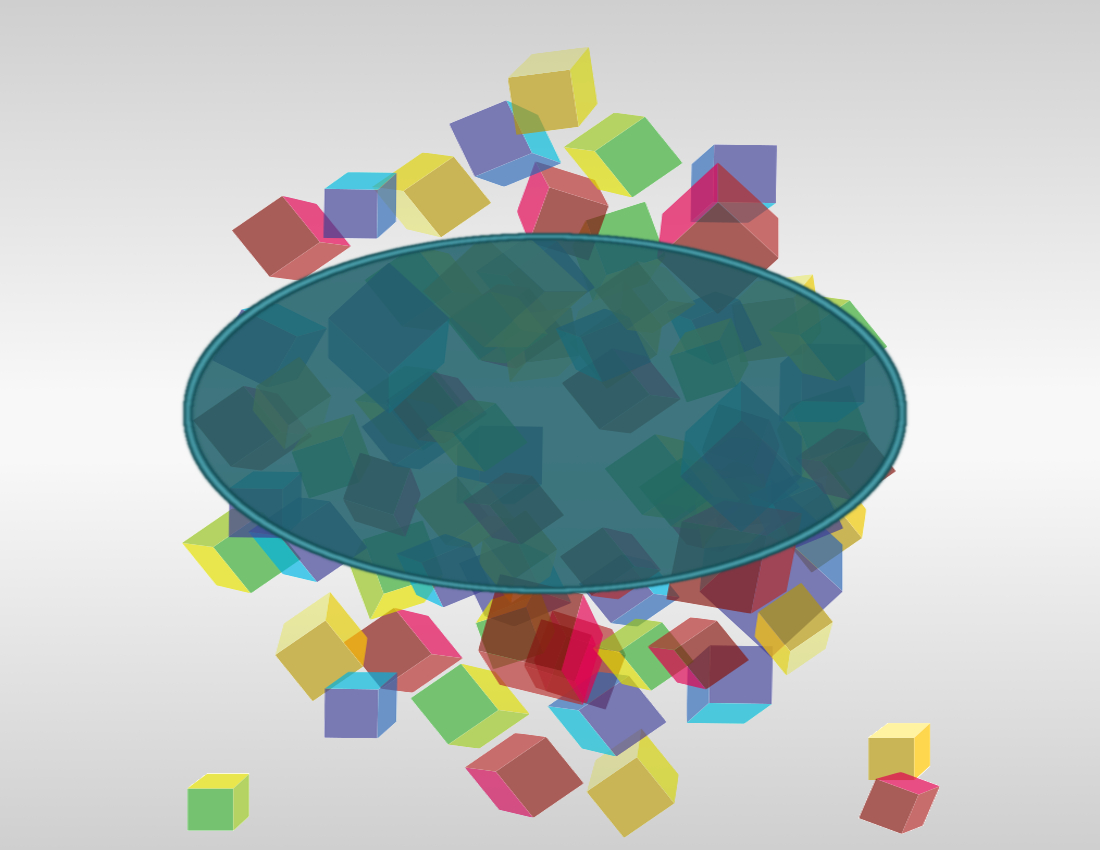
\includegraphics[width=11in,height=8.5in]{img/bg.jpg}
  }%
}

\definecolor{miazul}{RGB}{195, 227, 233}
\definecolor{miazul2}{RGB}{0, 51, 59}
\definecolor{miotroazul}{RGB}{15, 72, 80}
\graphicspath{{img/}}

\author{Jesús Mejía}



%\usepackage{helvet} \renewcommand{\familydefault}{\sfdefault}


\begin{document}
\BgThispage
\begin{minipage}{.15\textheight}

\includegraphics[scale=.35]{uv}
\end{minipage}
\begin{minipage}{.7\textheight}
\huge  \sc \centering \color{miazul2}
La Facultad de Matemáticas\\
de la Universidad Veracruzana
\end{minipage}
\begin{minipage}{.15\textheight}
\vspace*{.5cm}
\begin{flushright}

\includegraphics[scale=.4]{matematicas}
\end{flushright}
\end{minipage}
\begin{center} \color{miotroazul}
\rule{0.7\textwidth}{2px}\\[-3px]\rule{0.6\textwidth}{2px}
\end{center}
\vspace{1cm}

{\LARGE \it \sl Otorga la presente\\}
\begin{center}
\Huge \color{miazul}
\rule{0.65\textwidth}{3px}\\[5px]
{\sc \fontsize{45}{60}\selectfont  C o n s t a n c i a}\\[-20px]
\rule{0.65\textwidth}{3px}
\end{center}
%\vspace{1cm}
{\Large \sl Al:}
\begin{center}
\color{miazul}
\Huge \sc \fontsize{30}{60}\selectfont{
C. Nombre del Interesado}
\end{center}
\vspace{3cm}
\begin{center}
\LARGE   Por haber asistido al 1er. Taller de {\rm \LaTeX} realizado del 24 de agosto al 4 de septiembre de 2015.
\end{center}
\vspace{2cm}
\hspace{1cm}
\centering
\begin{minipage}{.4\textwidth}
\centering
\hrule
firma 1
\end{minipage}
\hspace{1cm}
\begin{minipage}{.4\textwidth}
\centering
\hrule
firma 2
\end{minipage}















 

\end{document}
